\documentclass{beamer}
\usepackage{graphicx}
\usepackage{hyperref}

\usecolortheme[named=orange]{structure}
\setbeamertemplate{navigation symbols}{}
\setbeamertemplate{footline}[frame number]
\setbeamercolor{framesubtitle}{fg=darkgray}
\title{Data \& Analytics Case Study}
\author{Max van Rooijen (max@pl9.co)}
\date{\today}
\titlegraphic{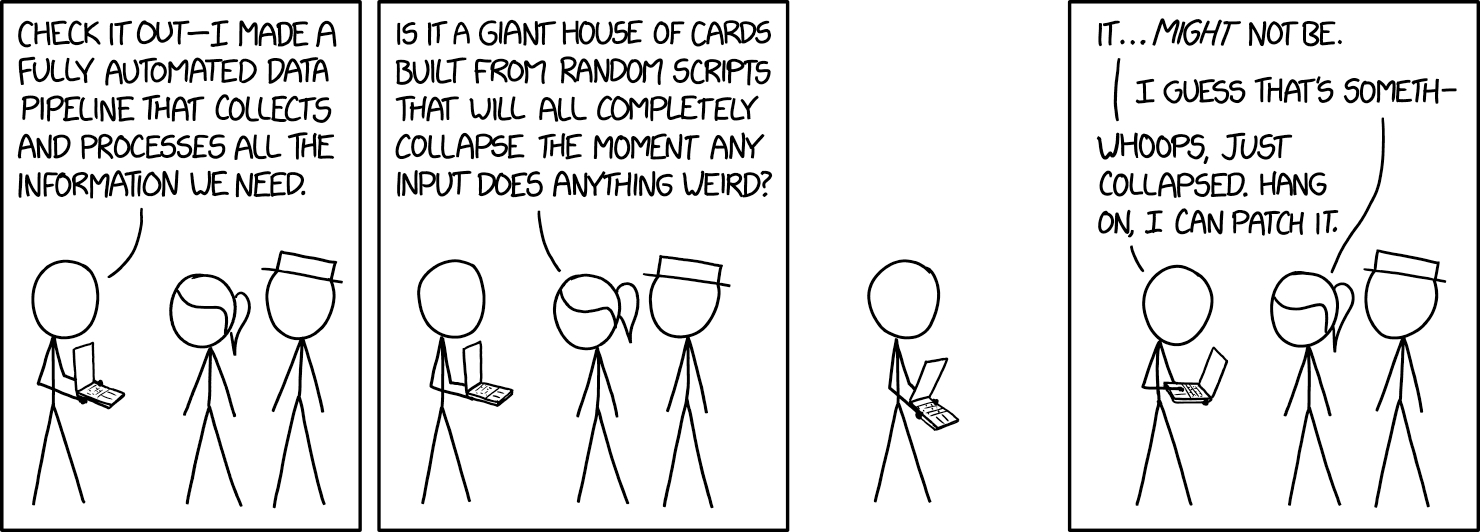
\includegraphics[width=0.9\textwidth]{../screenshots/data_pipeline_2x.png}}
% https://www.explainxkcd.com/wiki/index.php/2054:_Data_Pipeline

\begin{document}

\frame{\titlepage}

\section{Why: The Need for Analytics in Comic Design}
\begin{frame}{Why Analytics in Comic Design?}
    \begin{columns}
        \column{0.5\textwidth}
        \begin{itemize}
            \item Understanding audience preferences and engagement
            \item Optimizing storytelling and visual elementsd, see what works and what doesn't
            \item Enhancing content based on costs, views and reviews
        \end{itemize}
        \column{0.5\textwidth}
        \centering
        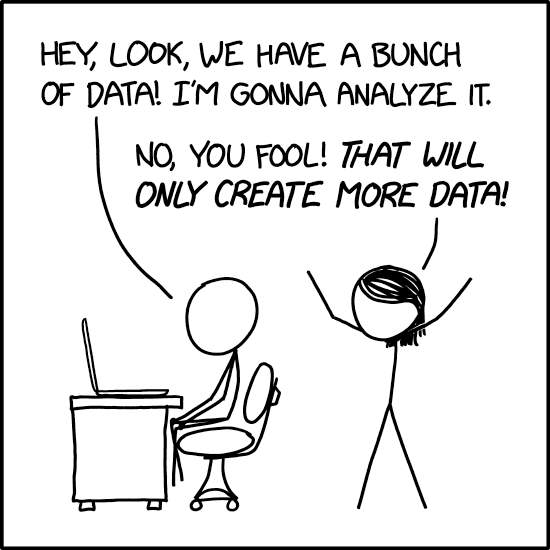
\includegraphics[width=0.9\textwidth]{../screenshots/data_trap_2x.png}
    \end{columns}
\end{frame}

\begin{frame}[t]{Technical Solution: Batch Processing Pipeline}
\framesubtitle{The How}
\raggedright
    The overall data pipeline executes these tasks:
    \begin{itemize}
        \item Fetching data from the XKCD API
        \item Using Apache Airflow to orchestrate workflows
        \item Staging data in a PostgreSQL Data Warehouse
        \item Transforming raw data using \textit{dbt}
        \item Running data quality checks to ensure integrity
    \end{itemize}
    \vspace{1em}
    Technologies used:
    \begin{itemize}
        \item \textbf{Apache Airflow}: To orchestrate workflows.
        \item \textbf{PostgreSQL}: For staging data in a Data Warehouse.
        \item \textbf{dbt (data build tool)}: For transforming raw data.
    \end{itemize}

\end{frame}

\begin{frame}{Solution Overview}
    \centering
    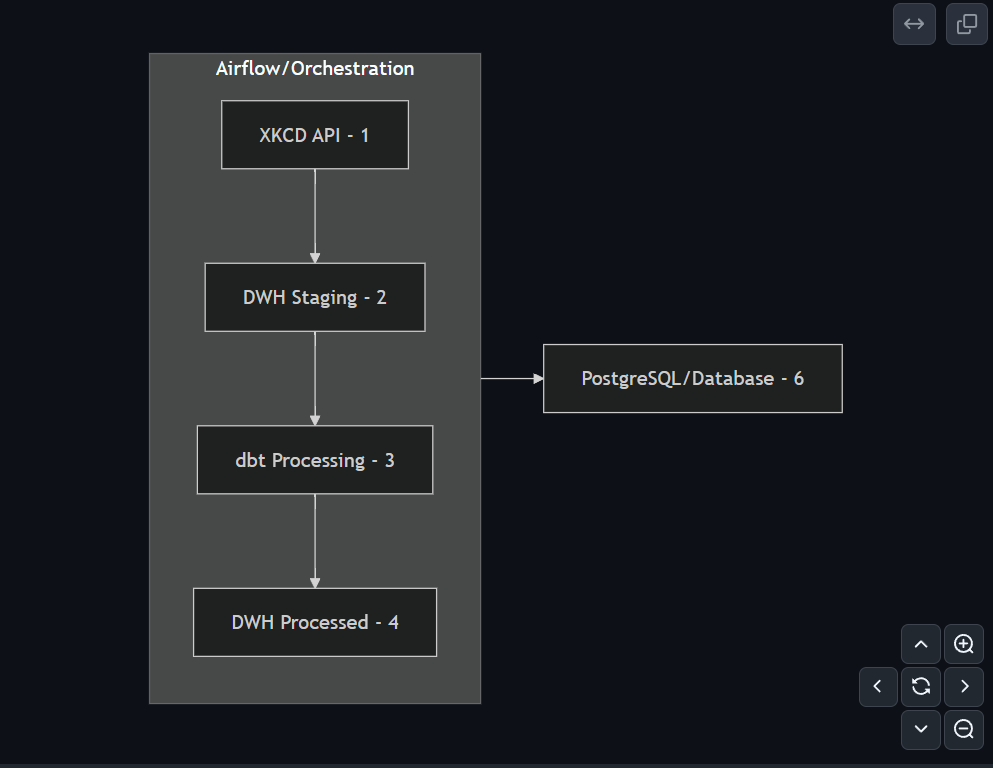
\includegraphics[width=0.8\textwidth]{../screenshots/solution_overview.png}
    \newline
    High-level overview of the architecture.
\end{frame}

\begin{frame}{Pipeline Architecture}
    \centering
    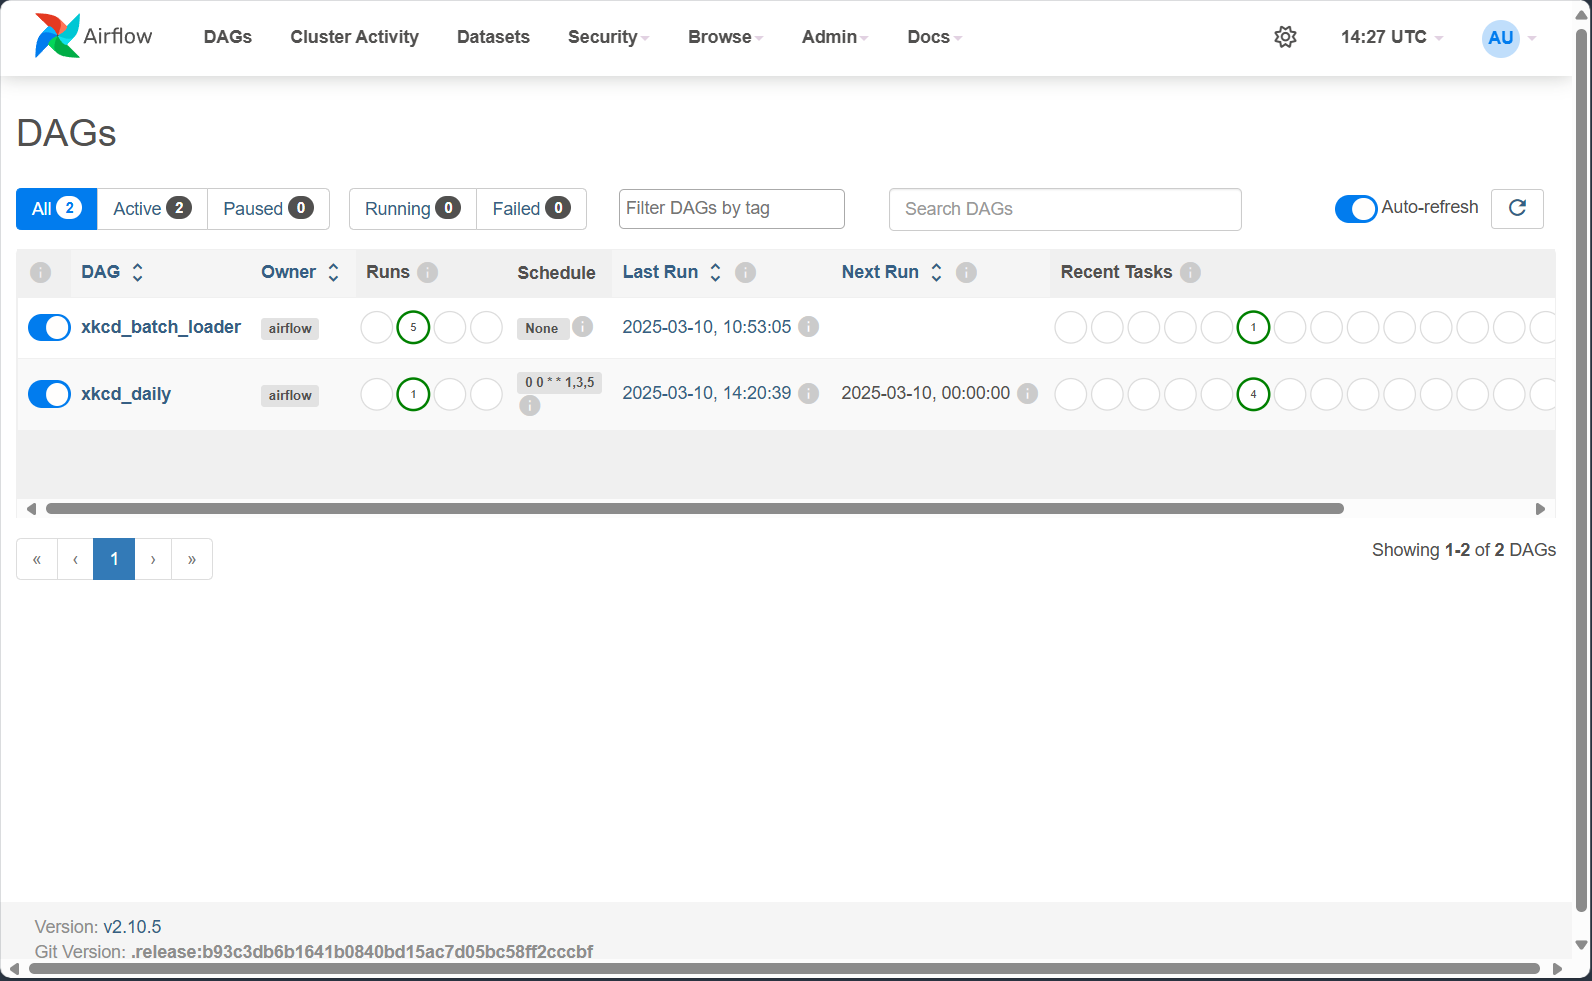
\includegraphics[width=0.8\textwidth]{../screenshots/airflow.png}
    \newline
    Overview of the DAGs in Airflow
\end{frame}

\begin{frame}{Pipeline Architecture}
    \centering
    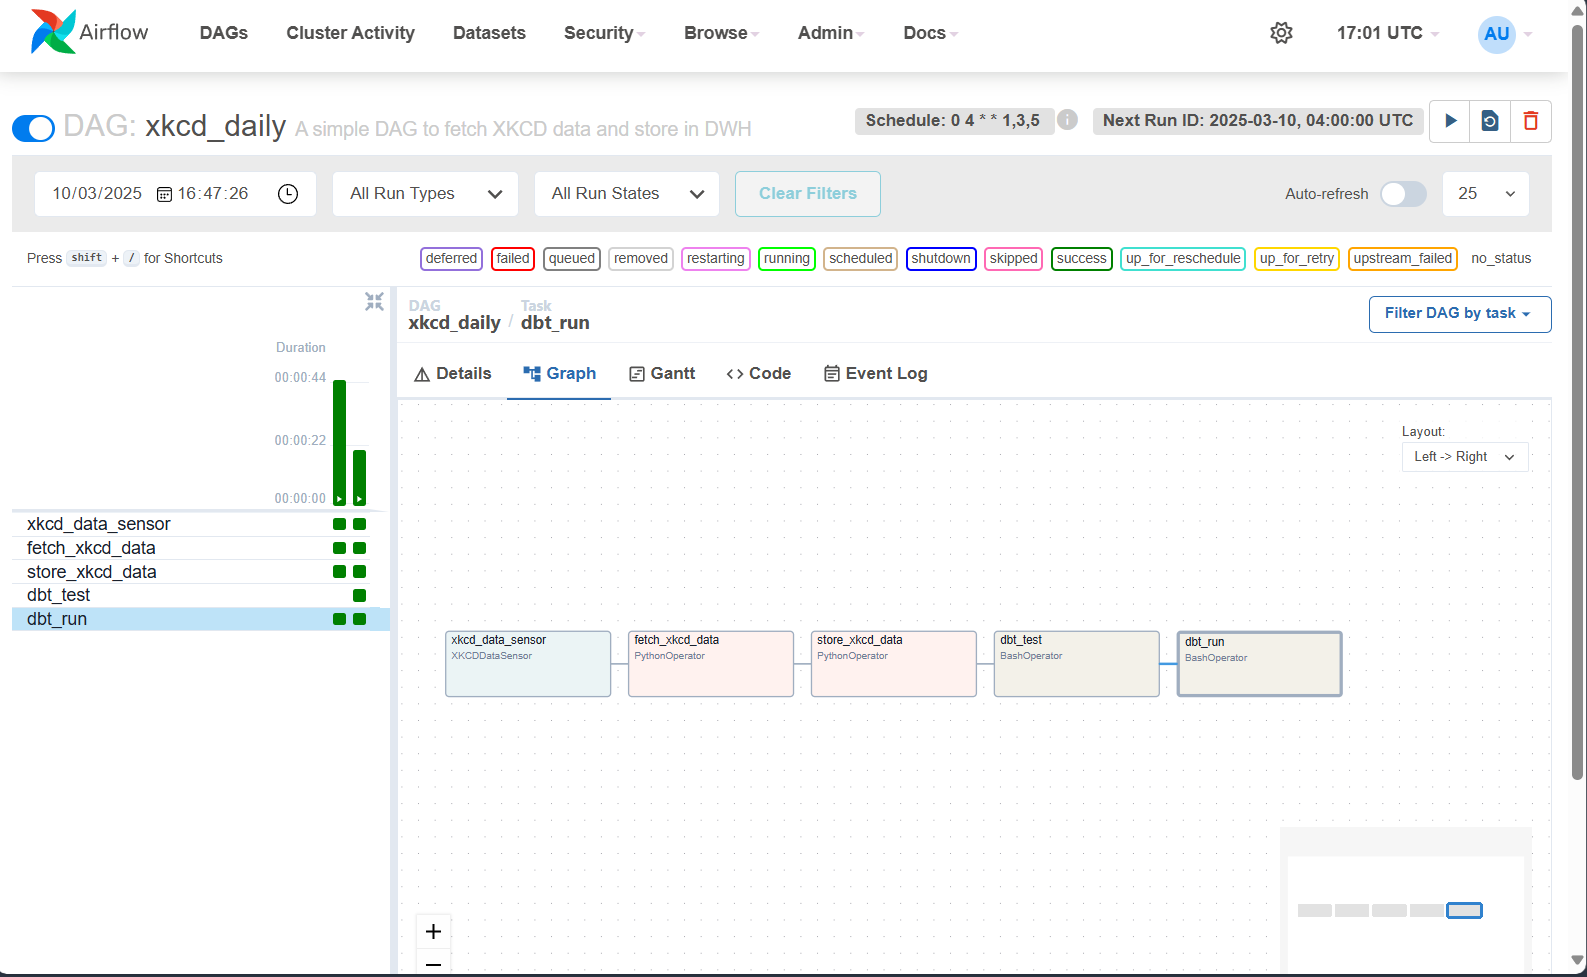
\includegraphics[width=0.8\textwidth]{../screenshots/airflow-dag.png}
    \newline
    Daily run DAG
\end{frame}

\begin{frame}{Data Model and Insights}
    \begin{itemize}
        \item Dimensional model for structured data storage
        \item Fact tables for costs, reviews, and views
        \item Aggregated insights for trend analysis
    \end{itemize}
    \centering
    \vspace{5em}
    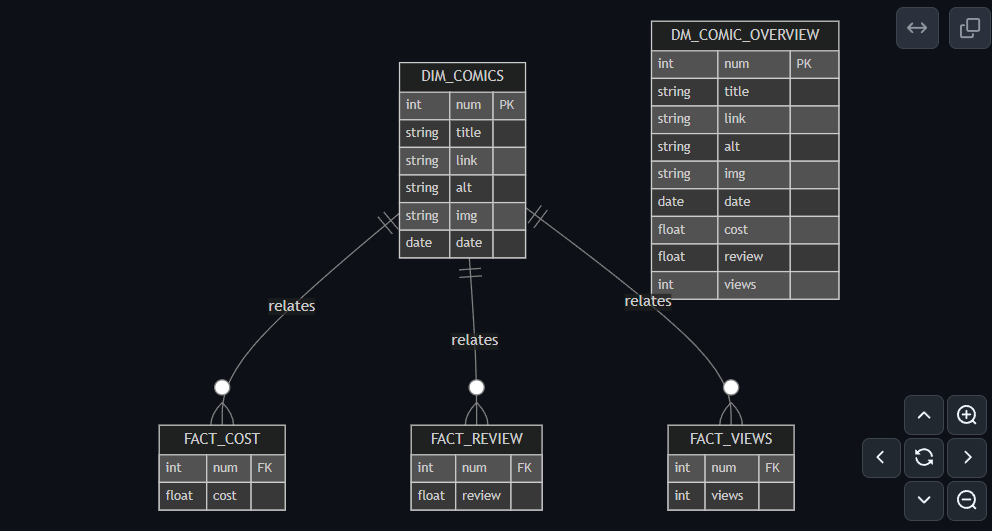
\includegraphics[width=0.8\textwidth]{../screenshots/er-diagram.png}
\end{frame}

\begin{frame}{Future Technical Improvements}
    \begin{itemize}
        \item \textbf{Machine Learning Integration}: Use ML models for predictive insights, such as forecasting trends in comic engagement.
        \item \textbf{Enhanced Data Quality Checks}: Implement more comprehensive tests for duplicates, referential integrity, and outlier detection.
        \item \textbf{Unit Tests for DAGs}: Add unit tests to Airflow DAGs to ensure robust workflow execution.
        \item \textbf{More Elaborate Data Model}: Expand the data warehouse schema to include more detailed metadata and user behavior analytics.
        \item \textbf{Scalability}: Optimize the data pipeline to handle larger volumes of data and improve performance.
        \item \textbf{Data Lineage}: Implement the dbt docs routine to automatically generate an interactive document in HTML and host it on a web server.
    \end{itemize}
\end{frame}

\section{Research Questions}
\begin{frame}{Research Questions}
    \small
    \begin{itemize}
        \item Which comics have the highest engagement rates and why?
        \item How do different types of content (e.g., tech, society) perform in terms of views and shares?
        \item What is the cost per engagement for the comics?
        \item Are there any trends in reader preferences over time?
        \item What are the common themes in reader feedback and reviews?
        \item How can we optimize our content strategy to increase reader retention and engagement?
        \item How does reader engagement correlate with revenue from ads and t-shirt sales?
    \end{itemize}
    \centering
    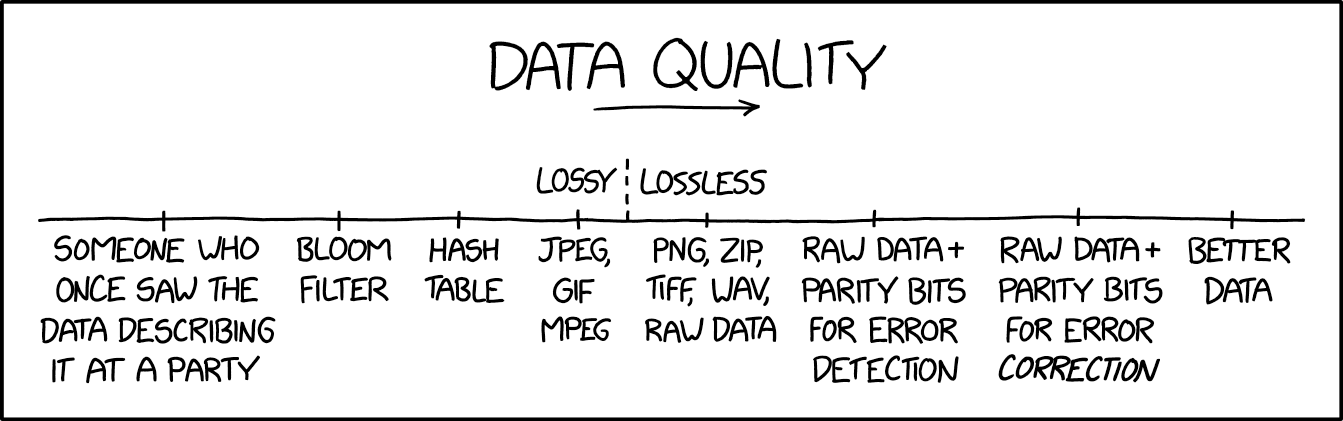
\includegraphics[width=0.8\textwidth]{../screenshots/data_quality_2x.png}
\end{frame}

\section{Future: Business Cases and Opportunities}
\begin{frame}{Future Business Cases}
    \centering
    
\includegraphics[width=0.4\textwidth]{../screenshots/scrooge.png}
    \begin{itemize}
        \item \textbf{Optimizing Ad Placement}: Use insights from user engagement to strategically place advertisements in comics.
        \item \textbf{Subscription \& Monetization Strategies}: Identify premium content opportunities based on engagement trends.
        \item \textbf{Predicting Viral Content}: Utilize data to forecast which comics are likely to go viral and maximize their exposure.
        \item \textbf{Improving Reader Retention}: Track engagement metrics to refine content strategy and keep readers coming back.
    \end{itemize}
\end{frame}

\end{document}
